\section{Лекция 16.01.2020}

\subsection{Линейные отображения векторных пространств}

Пусть $V$, $W$ --- векторные пространства над $F$.

\begin{definition}
    Отображение $\phi \colon V \to W$ называется \textit{линейным}, если
    \begin{enumerate}
    \item \label{lec16:def_1_1}$\phi(v_1 + v_2) = \phi(v_1) + \phi(v_2)$,
    \item \label{lec16:def_1_2} $\phi(\lambda v) = \lambda \phi(v)$.
    \end{enumerate}

    $\forall v_1, v_2, v \in V$, $\forall \lambda \in F$.
\end{definition}

\begin{exercise}
    \ref{lec16:def_1_1} и \ref{lec16:def_1_2} эквивалентны тому, что 

    $\phi(\lambda_1 v_1 + \lambda_2 v_2) = \lambda_1 \phi(v_1) + \lambda_2 \phi(v_2)$.

    $\forall v_1, v_2 \in V$, $\forall \lambda_1, \lambda_2 \in F$.
\end{exercise}

\subsection{Примеры линейных отображений}

\href{https://www.dropbox.com/s/t2or1ihptvg7xe6/LM_examples.pdf?dl=0}{Презентация} (продублирована ниже)

\subsubsection{Пример 0}

$\phi\colon V \to W$ --- нулевое отображение,

$\phi(v) := \overrightarrow{0} \quad \forall v \in V$

\bigskip
\begin{enumerate}[label=\arabic*), nosep]
\item $\phi(v_1 + v_2) = \overrightarrow{0} = \overrightarrow{0} + \overrightarrow{0} = \phi(v_1) + \phi(v_2)$,
\item $\phi(\lambda \cdot v) = \overrightarrow{0} = \lambda \overrightarrow{0} = \lambda \cdot \phi(v)$.
\end{enumerate}

\subsubsection{Пример 1}

$\phi\colon V \to V$ --- тождественное отображение,

$\phi(v) := v \quad \forall v \in V$.

Обозначение: $\phi =: \text{Id}$.

\bigskip
\begin{enumerate}[label=\arabic*), nosep]
\item $\phi(v_1 + v_2) = v_1 + v_2 = \phi(v_1) + \phi(v_2)$,
\item $\phi(\lambda \cdot v) = \lambda \cdot v = \lambda \cdot \phi(v)$.
\end{enumerate}

\subsubsection{Пример 2}

$\phi\colon \RR^2 \to \RR^2$ --- поворот на угол $\alpha$ вокруг начала координат. 

\bigskip
Два красных вектора $v_1$, $v_2$ и их сумму $v_1 + v_2$ повернули на угол $\alpha$, получив $\phi(v_1)$, $\phi(v_2)$ а так же точку $A$.

Свойство $1$ говорит нам, что точка $A$ это не просто сумма образов, она так же является образом суммы $v_1 + v_2$.

То есть точку $A$ можно получить двумя разными способами: сложить $\phi(v_1)$ и $\phi(v_2)$ или повернуть $v_1 + v_2$.

\bigskip
Вторая картинка показывает свойство $2$: точка $B$ это с одной стороны $\phi(v) \cdot \lambda$, а с другой --- образ $\lambda \cdot v$. 

\begin{center}
    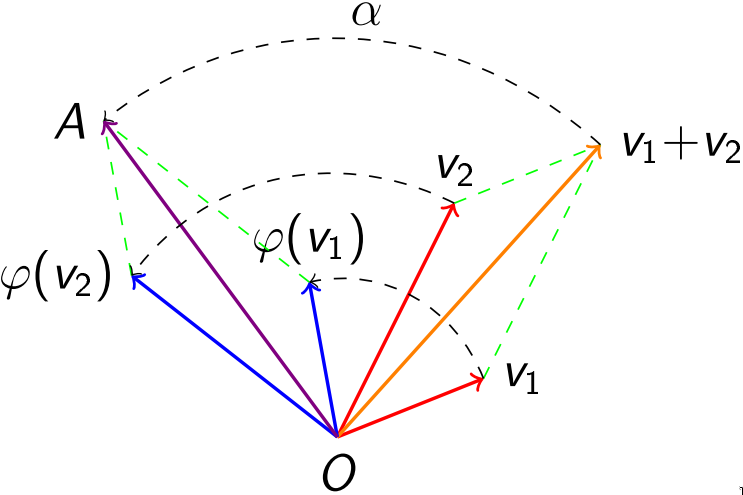
\includegraphics[height=5cm]{img/lecture16_example2_1}
    \hspace{2cm}
    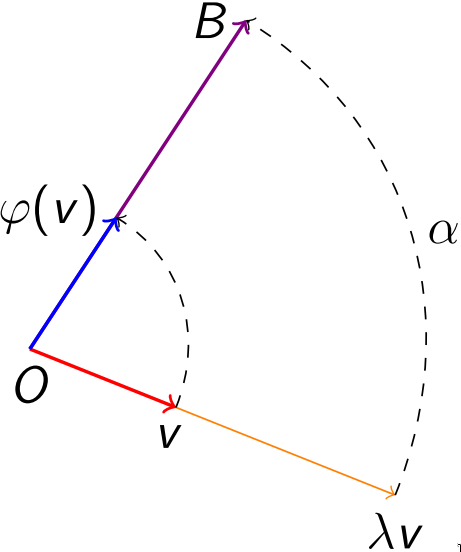
\includegraphics[height=5cm]{img/lecture16_example2_2}
\end{center}

\bigskip
\begin{enumerate}[label=\arabic*), nosep]
\item $\phi(v_1) + \phi(v_2) = A = \phi(v_1 + v_2)$,
\item $\phi(\lambda \cdot v) = B = \lambda \cdot \phi(v)$.
\end{enumerate}

\subsubsection{Пример 3}

$\phi\colon \RR^3 \to \RR^2$ --- ортогональная проекция на плоскость $Oxy$.

\begin{center}
    $\langle$ Конкурс на лучшую картинку $\rangle$
\end{center}

\subsubsection{Пример 4}

$\RR[x]_{\leq n}$ --- пространство многочленов от $x$ степени $\leq n$ с коэффициентами из $\RR$.

$\Delta \colon f(x) \mapsto f'(x)$ --- отображение дифференциирования.

\bigskip
\begin{enumerate}[label=\arabic*), nosep]
\item \label{lec16:example4_1} $(f + g)' = f' + g'$,
\item \label{lec16:example4_2} $(\lambda \cdot f)' = \lambda \cdot f' \quad \forall \lambda \in \RR$.
\end{enumerate}

\bigskip
\ref{lec16:example4_1} и \ref{lec16:example4_2} $\implies \Delta $ --- линейное отображение $\RR[x]_{\leq n} \to \RR[x]_{\leq n - 1}$.

\subsubsection{Пример 5}
\label{lec16:example_5}

$V$ --- векторное пространство над $F$, $\dim V = n$.

$(e_1, \dots, e_n)$ --- базис $V$.

$\phi \colon V \to F^n$

$v = x_1 e_1 + \dots + x_n e_n \implies \phi(v) := \begin{pmatrix} x_1 \\ \vdots \\ x_n \end{pmatrix}$.

Покажем, что оно линейно:

Пусть \begin{equation*}
    v = x_1 e_1 + \dots + x_n e_n \implies \phi(v) := \begin{pmatrix} x_1 \\ \vdots \\ x_n \end{pmatrix}
,\end{equation*} 
\begin{equation*}
    w = y_1 e_1 + \dots + y_n e_n \implies \phi(w) = \begin{pmatrix} y_1 \\ \vdots \\ y_n \end{pmatrix}
.\end{equation*}

Тогда,
\begin{enumerate}[label=\arabic*), nosep]
    \item \label{lec16:example5_1} $v + w = (x_1 + y_1) e_1 + \dots + (x_n + y_n) e_n \implies \phi(v + w) = \begin{pmatrix} x_1 + y_1 \\ \vdots \\ x_n + y_n \end{pmatrix} = \begin{pmatrix} x_1 \\ \vdots \\ x_n \end{pmatrix} + \begin{pmatrix} y_1 \\ \vdots \\ y_n \end{pmatrix} = \phi(v) + \phi(w)$,
    \item \label{lec16:example5_2} $\lambda \cdot v = (\lambda x_1) e_1 + \dots + (\lambda x_n) e_n \implies \phi(\lambda \cdot v) = \begin{pmatrix} \lambda x_1 \\ \vdots \\ \lambda x_n \end{pmatrix} = \lambda \begin{pmatrix} x_1 \\ \vdots \\ x_n \end{pmatrix} = \lambda \phi(v)$.
\end{enumerate}

\subsection{Простейшие свойства линейных отображений}

Здесь $\overrightarrow{0_V}$ --- нулевой вектор в векторном пространстве $V$.

\begin{enumerate}
\item $\phi(\overrightarrow{0_V}) = \overrightarrow{0_W}$.

    Доказательство: $\phi(\overrightarrow{0_V}) = \phi(0 \cdot \overrightarrow{0_V}) = 0 \cdot \phi(\overrightarrow{0_V}) = \overrightarrow{0_W}$.

\item $\phi(-v) = -\phi(v)$.

    Доказательство: $\phi(-v) + \phi(v) = \phi(-v + v) = \phi(0) = \phi(\overrightarrow{0_V)} = \overrightarrow{0_W} \implies \phi(-v) = -\phi(v)$.
\end{enumerate}


\subsection{Изоморфизм векторных пространств}

\begin{definition}
    Отображение $\phi \colon V \to W$ называется \textit{изоморфизмом} если оно линейно и биективно.

    Обозначение: $\phi \colon V \MapsTo W$.
\end{definition}

В примерах выше:
\begin{enumerate}[nosep]
\setcounter{enumi}{-1}
\item $\phi$ --- изоморфизм $\iff \begin{cases}
    V = \{\overrightarrow{0}\}, \\
    W = \{\overrightarrow{0}\}
\end{cases}$

\item да
\item да
\item нет
\item $\phi$ --- изоморфизм $\iff n = 0$
\item да!
\end{enumerate}


\subsection{Отображение, обратное к изоморфизму}

\begin{proposal}
    \label{lec16:prop_1}
    Если $\phi \colon V \to W$ --- изоморфизм, то $\phi^{-1}$ --- тоже изоморфизм. 
\end{proposal}

\begin{proof}
    Биективность есть, так как $\phi^{-1}$ --- обратное отображение.

    Проверим линейность
    \begin{enumerate}[label=\arabic*)]
    \item $w_1, w_2 \in W \implies w_1 = \phi(\phi^{-1}(w_1))$, $w_2 = \phi(\phi^{-1}(w_2))$
        \begin{align*}
            \phi^{-1}(w_1 + w_2) &= \phi^{-1}\Big(\underbrace{\phi\left(\phi^{-1}(w_1)\right)}_{w_1} + \underbrace{\phi\left(\phi^{-1}(w_2)\right)}_{w_2}\Big) \\
            &= \underbrace{\phi^{-1}\big(\phi}_{Id}\left(\phi^{-1}(w_1) + \phi^{-1}(w_2)\right)\!\big)\\
            &= \phi^{-1}(w_1) + \phi^{-1}(w_2)
        .\end{align*}

    \item 
        \begin{align*}
            \phi^{-1}(\lambda \cdot w_1) &= \phi^{-1}\left(\lambda \cdot \phi\left(\phi^{-1}\left(w_1\right)\right)\right) \\
            &= \underbrace{\phi^{-1}\big(\phi}_{Id}\left(\lambda \cdot \phi^{-1}(w_1)\right)\!\big) \\
            &= \lambda \phi^{-1}(w_1)
        .\qedhere\end{align*}
    \end{enumerate}
\end{proof}


\subsection{Композиция двух линейных отображений, композиция двух изоморфизмов}

Пусть $U \xrightarrow{\psi} V \xrightarrow{\phi} W$, тогда $\phi \circ \psi : U \to W$ --- композиция.

\begin{proposal}~
    \label{lec16:prop_2}
    \begin{enumerate}[nosep]
    \item Если $\phi$, $\psi$ линейны, то $\phi \circ \psi$ тоже линейна.
    \item Если $\phi$, $\psi$ --- изоморфизмы, то $\phi \circ \psi$ --- тоже изоморфизм.
    \end{enumerate}
\end{proposal}

\begin{proof}~
    \begin{enumerate}
    \item \label{lec16:comp_1}
        \begin{enumerate}[label=(\arabic*)]
            \item $(\phi \circ \psi)(u_1 + u_2) = \phi(\psi(u_1 + u_2)) = \phi(\psi(u_1) + \psi(u_2)) = \phi(\psi(u_1)) + \phi(\psi(u_2)) = (\phi \circ \psi)(u_1) + (\phi \circ \psi)(u_2)$.
            \item $(\phi \circ \psi)(\lambda u) = \phi(\psi(\lambda u)) = \phi(\lambda \psi(u)) = \lambda \phi(\psi(u)) = \lambda(\phi \circ \psi)(u)$.
        \end{enumerate}
    \item из \ref{lec16:comp_1} следует, что $(\phi \circ \psi)$ линейно, но при этом биективно как композиция двух биекций.
        \qedhere
    \end{enumerate}
\end{proof}


\subsection{Изоморфные векторные пространства}

\begin{definition}
    Два векторных пространства $V$, $W$ называются \textit{изоморфными}, если существует изоморфизм \\ ${\phi\colon V \MapsTo W}$.

    Обозначается: $V \simeq W$ (либо $V \cong W$).
\end{definition}


\subsection{Отношение изоморфности на множестве всех векторных пространств}

\begin{theorem}
    Отношение изоморфности является отношением эквивалентности на множестве всех векторных пространств над фиксированным полем $F$.
\end{theorem}

\begin{proof}~
    \begin{enumerate}
    \item Рефлексивность: $Id: V \MapsTo V$.
    \item Симметричность: $V \simeq W \implies W \simeq V$ следует из \hyperref[lec16:prop_1]{Предложения 1}.
    \item Транзитивность: $U \simeq V$, $V \simeq W \implies U \simeq W$ следует из \hyperref[lec16:prop_2]{Предложения 2}.
        \qedhere
    \end{enumerate}
\end{proof}


\subsection{Классы изоморфизма векторных пространств}

\begin{definition}
    Классы эквивалентности называются \textit{классами изоморфизма}.   
\end{definition}

\begin{example}
    $F[x]_{\leq n} \simeq F^{n + 1}$:

    $a_0 + a_1 x + \dots + a_n x^n \longleftrightarrow \begin{pmatrix} a_0 \\ a_1 \\ \vdots \\ a_n \end{pmatrix}$.
\end{example}


\subsection{Критерий изоморфности двух конечномерных векторных пространств}

\begin{theorem}
    Пусть $V$, $W$ --- два конечномерных векторных пространства над $F$.

    Тогда, $V \simeq W \iff \dim V = \dim W$.
\end{theorem}

\begin{lemma}
    \label{lec16:lemma_1}
    $\dim V = n \implies V \simeq F^n$.
\end{lemma}

\begin{proof}
    Фиксируем базис $(e_1, \dots, e_n)$ в $V$.

    Тогда, отображение $\phi \colon V \to F^n$ из \hyperref[lec16:example_5]{Примера 5} --- изоморфизм.
\end{proof}

\begin{lemma}
    \label{lec16:lemma_2}
    Пусть $\phi \colon V \MapsTo W$ и $e_1, \dots, e_n$ --- базис $V$, тогда $\phi(e_1), \dots, \phi(e_n)$ --- базис $W$. 
\end{lemma}

\begin{proof}
    Пусть $w \in W$. Тогда $\exists x_1, \dots, x_n \in F$, такие что $\phi^{-1}(w) = x_1 e_1 + \dots + x_n e_n$.

    Тогда, $w = \phi\left(\phi^{-1}(w)\right) = \phi(x_1 e_1 + \dots + x_n e_n) = x_1 \phi(e_1) + \dots + x_n \phi(e_n) \implies W = \langle \phi(e_1), \dots, \phi(e_n) \rangle$.

    Теперь докажем линейную независимость:

    Пусть $\alpha_1 \phi(e_1) + \dots + \alpha_n \phi(e_n) = \overrightarrow{0}$.

    Тогда, $\phi(\alpha_1 e_1 + \dots + \alpha_n e_n) = \overrightarrow{0}$.

    Применяя $\phi^{-1}$ получаем, $\alpha_1 e_1 + \dots + \alpha_n e_n = \phi^{-1}(\overrightarrow{0}) = \overrightarrow{0}$. Значит, $\alpha_1 = \dots = \alpha_n = 0$.

    Итог: $\phi(e_1), \dots, \phi(e_n)$ --- базис в $V$.
\end{proof}

\begin{proof}[Доказательство теоремы]~
    \begin{description}
    \item[$\impliedby$] Пусть $\dim V= \dim W = n$. Тогда по \hyperref[lec16:lemma_1]{лемме 1} $V \simeq F^n, W \simeq F^n$, значит $V \simeq W$.
    \item[$\implies$] Пусть $V \simeq W$. Фиксируем изоморфизм $\phi \colon V \MapsTo W$.

        Тогда по \hyperref[lec16:lemma_2]{лемме 2} получаем, что $\phi(e_1), \dots, \phi(e_n)$ --- базис $W$, а значит $\dim V = n = \dim W$.
        \qedhere
    \end{description}
\end{proof}

\begin{exercise}
    Если $\dim V = n$, то все изоморфизмы $V \MapsTo F^n$ находятся в биекции с базисами пространства $V$.
\end{exercise}


\subsection{Задание линейного отображения путём задания образов векторов фиксированного базиса}

Пусть $V$, $W$ --- векторные пространства над $F$ и $(e_1, \dots, e_n)$ --- фиксированный базис в $V$.

\begin{proposal}~
    \label{lec16:propopop}
    \begin{enumerate}
    \item Если $\phi \colon V \to W$ --- линейное отображение, то $\phi$ однозначно определяется векторами $\phi(e_1), \dots, \phi(e_n)$,
    \item $\forall w_1, \dots, w_n \in W \ \exists!$ линейное отображение $\phi$, такое что, $\phi(e_1) = w_1, \dots, \phi(e_n) = w_n$.
    \end{enumerate}
\end{proposal}

\begin{proof}~
    \begin{enumerate}
    \item \label{lec16:kekek}
        $v \in V \implies v = x_1 e_1 + \dots + x_n e_n \implies \phi(v) = x_1 \phi(e_1) + \dots + x_n \phi(e_n)$.
    \item 
        Зададим $\phi \colon V \to W$ формулой $\phi(x_1 e_1 + \dots + x_n e_n) = x_1 w_1 + \dots + x_n w_n$.

        Тогда $\phi$ --- линейное отображение из $V$ в $W$ (упражнение).

        Единственность следует из \ref{lec16:kekek}
        \qedhere
    \end{enumerate}
\end{proof}
